\capitulo{5}{Aspectos relevantes del desarrollo del proyecto}

En este apartado se va a recoger el ciclo de vida del proyecto, detallando los aspectos más relevantes que se han tratado y como se han resuelto las diferentes dificultades encontradas a lo largo de su desarrollo. Se irán presentando diferentes secciones que concuerdan con el orden cronológico seguido en el proyecto y muestran la justificación de las decisiones tomadas.

\section{Propuesta del Proyecto}

La propuesta de este proyecto consistía en crear un modelo clasificador integrado en una iterfaz para el reconocimiento de materiales que se dividía en las siguientes 3 tareas principales:

\begin{itemize}
\item[•] \textbf{Montaje del sensor:} Puesta en funcionamiento del radar junto con sus componentes. Siendo capaces de extraer las características del las lecturas realizadas.

\item[•] \textbf{Lecturas de los materiales:} Conseguir información a través de las características de los materiales para crear un modelo capaz de diferenciar materiales como son: cartón, plástico y cristal.

\item[•] \textbf{Clasificador de materiales:} La tarea principal pedida para realizar este proyecto era la de construir un clasificador de materiales a través de un radar de 60GHz devolviendo la identificación correcta del material.
\end{itemize}

\section{Metodologias aplicadas}

En el desarrollo de este proyecto se ha intentado emplear en la medida de los posible la metodología ágil de \textit{Scrum}.

Debido a que el proyecto se comenzó en abril de 2021, no se ha podido seguir de forma estricta todas las pautas de la metodología, como las reuniones diarias con todo el equipo. 

Las pautas que se han seguido durante el proyecto han sido:
\begin{itemize}
\item Desarrollo incremental del proyecto mediante \textit{sprints}. 
\item \textit{Spints} de 1 a 2 semanas. 
\item Al finalizar el \textit{sprint}, reuniones para evaluar el proyecto y plantear los pasos a seguir en el siguiente \textit{sprint}.
\end{itemize}

\section{Formación}
Durante las primeras fases del proyecto, fue necesario aprender el funcionamiento del Radar Sensor. Para ello, se consultó la documentación facilitada por el fabricante \textit{Acconeer}.

A parte de esto se investigó información adicional sobre el uso de estos radares, así como ejemplos de su uso, la información extraída de la red fue escasa o casi nula. Únicamente fue válida la documentación facilitada por \href{https://acconeer-python-exploration.readthedocs.io/}{\textit{Acconeer}}.

\section{Montaje del radar}

En esta sección se indican tanto las necesidades hardware como software para el montaje y puesta en funcionamiento del radar.

\subsection{Necesidades hardware}
Los creadores de \textit{Acconner} han elaborado un vídeo (\href{https://www.youtube.com/watch?v=0uKrm_RAV_c}{\textit{EVK 2}}) con las instrucciones del montaje del sensor. En él se detallan los diferentes componentes y el montaje de hardware a la \textit{Raspberry Pi 4}.

En un comienzo será necesario disponer de: 
\begin{itemize}
	\item Raspberry Pi 4
	\item Radar A111
	\item Placa XR112
	\item Cable flexible para XR112
	\item Tarjeta SD
	\item Teclado USB
	\item Ratón USB
	\item Monitor con HDMI
	\item Cable HDMI
	\item Adaptador mini HDMI a HDMI
\end{itemize}

\imagen{componentes_radar}{Componentes principales}

La figura \ref{fig:componentes_radar} muestra los siguientes componentes:
\begin{itemize}
	\item[]\textbf{1 -} Radar A111
	\item[]\textbf{2 -} Raspberry Pi 4
	\item[]\textbf{3 -} Placa XR112
	\item[]\textbf{4 -} Cable flexible para XR112
\end{itemize}


La placa se conecta a la \textit{Raspberry} por el puerto \textit{GPIO} quedando por encima del resto.

\imagen{componentes_conectados}{Componentes en conexión}

Se ha realizado un espacio o cubículo de lectura de objetos de $30x22x25 cm$ (ancho, largo y alto) con una incisión en la parte superior, en el medio, del tamaño del sensor. El sensor fue bloqueado a su posición solamente colocándole en la posición de la incisión y sujetado con cinta adhesiva. Esta caja de madera se utiliza poniendo la abertura en la parte lateral, mirando al operario que hace uso del radar.
 
El sensor tiene sensibilidad a partir de los 10 cms. La sensibilidad del sensor se limitó al rango de 10 a 24 cm, el mínimo de sensibilidad hasta el suelo.

\imagen{prototipo}{Prototipo}

\subsection{Necesidades software}

Una vez se había procedido con el montaje del dispositivo se pasó a la instalación y configuración del sistema operativo. Además, se instalaron los diversos programas necesarios tanto para recoger los datos como para poder interpretarlos.

La tarjeta SD facilitada por la UBU ya disponía del sistema operativo necesario para realizar las lecturas, tras esto se debía comenzar a investigar como ejecutar el radar desde un cuaderno de Python.

Para realizar una instalación desde cero del radar serán necesarios los siguiente programa. Además, nos pueden resultar útiles a la hora de trabajar con el Radar. 
Hay que descargar e instalar: 
\begin{itemize}
\item \href{http://developer.acconeer.com}{\textit{Acconeer SW}}: disponible para todos los usuarios (\textit{Windows, Linux, iOS}) 
\item \href{www.raspberrypi.org}{\textit{Raspbian OS}} 
\item \href{http://www.etcher.io}{\textit{Etcher}}: se usará para instalar el sistema operativo \textit{Raspbian} en la tarjeta SD
\item \href{http://www.putty.org}{\textit{PuTTY}}: se utiliza para conectarse a \textit{Raspberry Pi}
\item \href{http://www.winscp.net}{\textit{WinSCP}}: utilizado para transferir archivos a la tarjeta SD
\end{itemize}
 
\section{Lectura de los objetos}

Para la creación del modelo se han seleccionado 30 materiales divididos en, 10 de plástico, 10 de cristal y 10 de cartón. De cada material se han realizado 10 lecturas, de varias caras, girando el objeto.

Llegamos a una colección de 300 lecturas exportadas cada una en ficheros con formato \textit{numpy} (.npy) donde están almacenadas las características en vectores y matrices. Un porcentaje de estos datos conformaran la red de entrenamiento y otro porcentaje servirán para testear la red.

Estas lecturas se han realizado desde el cuaderno de Jupyter «\href{https://github.com/mecyc/TFG_RADAR_60GHZ/scripts/LecturasRadar.ipynb}{LecturasRadar}».

\imagen{conf_acconeer}{Configuración inicial.}


Se ha establecido el radar con los siguientes parámetros:
\begin{itemize}
	\item[•]Indicamos el \textit{hostname} (RadarAcconeer) y el modo de conexión mediante \textit{socket}
	\item[•]Servicio IQ
	\item[•]Perfil 2 (distancias de unos 20 cm)
	\item[•]Tasa de lectura de 30 Hz
	\item[•]Normalización desactivada (solo se recomienda activada para representar datos)
	\item[•]Ganancia medio punto, la ganancia es la intensidad de la señal.
\end{itemize}

Una vez establecida la configuración debemos tener el radar encendido y conectado a la misma red que nuestro equipo. Tras esto vamos ejecutando el cuaderno para realizar las lecturas de los objetos. Como el intercambio de los objetos para la lectura es manual la ejecución del cuaderno también la haremos manual y tomando los tiempos oportunos.

Para poder obtener las lecturas debemos ejecutar el fichero indicado en la figura \ref{fig:consola_radar}. Esta obligatoriedad de iniciar el servicio del radar se ha implementado en el desarrollo creado para este proyecto facilitando la ejecución de las lecturas.

\imagen{consola_radar}{Terminal del radar.}


Cada instante de tiempo de la lectura comprende 291 atributos, de cada fichero obtenemos del orden de 300 instancias. Una instancia son estadísticas de los 291 atributos calculadas a partir de los aproximadamente 300 instantes de tiempo.

Una vez finalizadas las lecturas se procedió al procesado de los datos de cada lectura para finalmente unirlos en datos de entrenamiento y test.

Tenemos los siguientes datos:
\begin{itemize}
\item \textit{N} es el numero de lecturas (1 objeto se corresponde con 10 vistas)
\item \textit{M} son los instantes de tiempo
\item \textit{A} referencia a los atributos
\end{itemize}

Se creará la siguiente matriz:
\begin{equation}
	Matriz1 = (N \cdot M) \cdot A
\end{equation}
Es una matriz 2D $(N \cdot M,A)$

La extracción y creación de la matriz con los datos necesarios se realizará mediante \textit{Python}:

\begin{verbatim}
diccionario = np.load('C01_V01.npy',allow_pickle=True).item()
data = diccionario.get('sweep_data').get('data')
data = data.reshape(data.shape[0],data.shape[2])
\end{verbatim}

Los datos de la lectura tienen una parte real y otra imaginaria, a partir del array 2D anterior, se obtiene otro array 2D, con el doble de anchura.
Por ejemplo, si Matriz1 es de $ 300 x 291 $, se obtendrá otra matriz que comprende el modulo y la fase de $ 600 x 291 $. Así se obtiene el módulo del número complejo y la fase del número complejo.
El módulo será una matriz de $ 300 x 291 $ y la fase también.

\begin{verbatim}
	modulo = abs(data)
	fase = []
		for i in data:
			fila = []
			for j in i:
				fila.append(phase(j)) #Fase
			fase.append(fila)
   	 	fase = np.asarray(fase)
   	 	modulo_fase = np.concatenate((modulo, fase), axis=0)
\end{verbatim}

A partir de los datos del modulo y la fase se obtiene la media.
\begin{verbatim}
	traspuesta = np.transpose(modulo_fase)
	#Obtenemos la matriz traspuesta(291x600) de modulo_fase(600x291)

	#Separamos la traspuesta en modulo y fase
	t_modulo = traspuesta[:,:int(traspuesta.shape[1]/2)]
	t_fase = traspuesta[:,int(traspuesta.shape[1]/2):]
	media = []
	for i in t_modulo:
    	media.append(i.mean())
	for j in t_fase:
    	media.append(j.mean())
	#media -> medias modulo y fase
\end{verbatim}

Una vez obtenidos los datos de las lecturas se comenzó con la creación de cuatro modelos clasificadores que más adelante se usarán para realizar la clasificación de los materiales junto con el radar.

Dentro del repositorio de \textit{GitHub} del proyecto hay un fichero llamado \textit{GenerarParticiones.ipynb} que incluye el desarrollo de todas estas funciones así como comentarios incisivos.

\section{Modelo clasificador}
Para elegir el modelo a usar se tuvieron que tener en cuenta diferentes factores como el peso del modelo, su carga de computo y su precisión.

Se realizaron pruebas con los diferentes modelos \textit{Random Forest}, \textit{k-nearest neighbors (k-NN)}, \textit{Support Vector Machine (SVM)}, \textit{auto-sklearn} y \textit{TabPFN}. 

Todos los modelos mantienen el mismo patrón de ejecución realizando una validación cruzada manual.

A continuación se incluyen los resultados obtenidos de entrenar cada clasificador, el código desarrollado para cada modelo lo encontramos en el repositorio de proyecto \url{https://github.com/mecyc/TFG_RADAR_60GHZ/tree/main/scripts}.

\clearpage

\subsection{\textit{Random Forest}}

Con el método \textit{Random Forest} se ha llegado a una tasa de acierto del 86.33\% estableciendo el número de árboles en 100.

En la figura \ref{fig:matrizconfusion_RF} se muestra la correspondiente matriz de confusión, junto con con la tasa de acierto promedio después de haber entrenado al modelo. El test se ha realizado en 10 particiones de 30 ficheros cada partición siguiendo la linea de la validación cruzada.
\begin{figure}[h]
\begin{center}
	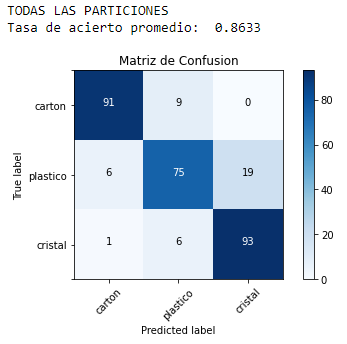
\includegraphics[scale=1.25]{matrizconfusion_RF}
	\caption{Matriz de confusión \textit{Random Forest}.}
	\label{fig:matrizconfusion_RF}
\end{center}
\end{figure}

Podemos ver que la confusión más frecuente son los objetos de plástico predichos erróneamente como cristal (19).

\clearpage

\subsection{\textit{k-NN}}

En la ejecución del clasificador \textit{k-NN} se ha decidido establecer un rango de 1 a 26 vecinos, rango que debería dar buenos resultados. Este método supone que los vecinos más cercanos nos dan la mejor clasificación y así ha sido, la mejor tasa de ha acierto ha sido con un vecino, una tasa del 87.67\%.

En la figura \ref{fig:matrizconfusion_KNN} se muestra la correspondiente matriz de confusión para 1 vecino. El rango de vecinos ha sido establecido de 1 a 26, el algoritmo en 1 vecino ha obtenido la mejor tasa de acierto.

\begin{figure}[h]
\begin{center}
	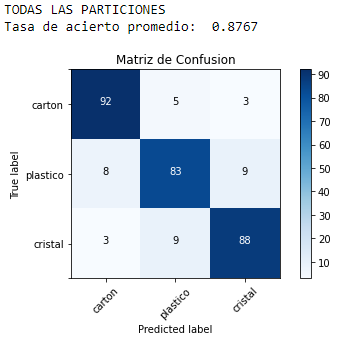
\includegraphics[scale=1.25]{matrizconfusion_KNN}
	\caption{Matriz de confusión \textit{k-NN}.}
	\label{fig:matrizconfusion_KNN}
\end{center}
\end{figure}

Según la gráfica de confusión obtenida vemos que los resultados son bastante parejos, obteniendo el mayor acierto en el cartón pero las confusiones son parejas entre los tres materiales. No ha sido la mayor tasa de acierto obtenida pero podemos decir que es la matriz de confusión con la diagonal más uniforme.

\clearpage

Gráfico que muestra la evolución del clasificador en el rango de 1 a 26 vecinos:

\imagen{grafica_KNN}{Evolución clasificador \textit{k-NN}.}

\clearpage

\subsection{\textit{SVM}}

En la ejecución del clasificador \textit{SVM} se ha decidido utilizar la clase \textit{GridSearchCV} para la búsqueda de parámetros. La tasa de acierto obtenida ha sido del 84.67\%.

\begin{figure}[h]
\begin{center}
	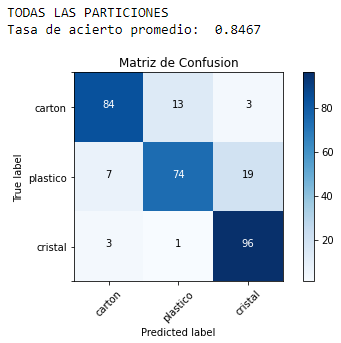
\includegraphics[scale=1.25]{matrizconfusion_SVM}
	\caption{Matriz de confusión \textit{SVM}.}
	\label{fig:matrizconfusion_SVM}
\end{center}
\end{figure}

\textit{SVM} nos da la matriz de confusión con menos tasa de acierto de los clasificadores utilizados. Obtiene una gran tasa de acierto en el cristal pero a la vez mantiene una confusión elevada al predecir el plástico (19) y el cartón (13).
\clearpage

\subsection{\textit{auto-sklearn}}

En la ejecución del clasificador \textit{auto-sklearn} se ha establecido el límite de tiempo para la búsqueda de modelo en 30 segundos y el límite para cada llamada en 120 segundos, ejecutando el modelo aumentando los segundos no ha mejorado la tasa de acierto. La tasa de acierto obtenida ha sido del 88\%

\begin{figure}[h]
\begin{center}
	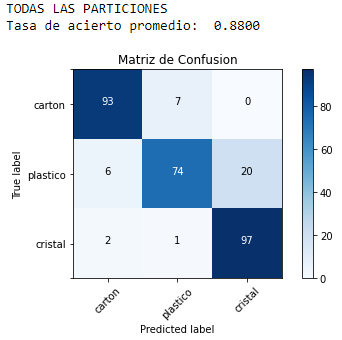
\includegraphics[scale=1.25]{matrizconfusion_AS}
	\caption{Matriz de confusión \textit{auto-sklearn}.}
	\label{fig:matrizconfusion_AS}
\end{center}
\end{figure}

Muestra una matriz de confusión muy parecida a la de \textit{Random Forest}, un acierto muy elevado en el cartón y cristal pero en el plástico mantiene 20 predicciones confusas.

\clearpage

\subsection{\textit{TabPFN}}

\textit{TabPFN} ha sido el último modelo incluido en el proyecto así como el más novedoso. Debido a la limitación de 100 características que presenta se ha decidido utilizar \textit{Pipeline} de \textit{Sklearn} para reducir de 582 características a 100. \textit{Pipeline} es una secuencia de mecanismos de procesamiento de datos.

\textit{LogisticRegression} es el modelo escogido para que \textit{Pipeline} seleccione las 100 características para entrenar a \textit{TabPFN}.

La tasa media de acierto obtenida ha sido la mejor hasta el momento llegando al 90\%.

\begin{figure}[h]
\begin{center}
	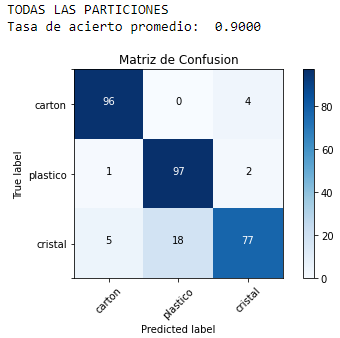
\includegraphics[scale=1.25]{matrizconfusion_TabPFN}
	\caption{Matriz de confusión \textit{TabPFN}.}
	\label{fig:matrizconfusion_TabPFN}
\end{center}
\end{figure}

\textit{TabPFN} nos ha dado la mayor tasa de acierto pero a decir verdad la matriz de confusión no ha sido la esperada, la confusión de indicar plástico (18) al cristal ha sido demasiado frecuente.
\clearpage

\subsection{Comparativa de clasificadores}

Viendo en la tabla \ref{tab:comparativa} se puede decir que en todos los modelos de clasificación hemos obtenido una tasa de acierto entre el 80\% y 90\% sin obtener unos resultados muy dispares.

\begin{table}[h]
\begin{center}
\begin{tabular}{l|c}
\hline
\rowcolor[gray]{0.9} 
\textbf{Modelo} & \textbf{Tasa de acierto (\%)} \\ \hline
\textit{Random Forest}   & 86.33                         \\ 
\rowcolor[gray]{0.9} 
\textit{k-NN}            & 87.67                         \\ 
\textit{SVM}             & 84.67                         \\ 
\rowcolor[gray]{0.9} 
\textit{auto-sklearn}    & 88                            \\ 
\textit{TabPFN}          & 90                            \\ \hline
\end{tabular}
\caption{Comparativa de modelos clasificadores.}
\label{tab:comparativa}
\end{center}
\end{table}

En nuestro caso, el método más sencillo (\textit{k-NN}) ha proporcionado resultados competitivos, hasta el punto de ser el tercer mejor método. \textit{Auto-sklearn} ha obtenido el segundo mejor resultado con el 88\%. El mejor resultado lo ha dado \textit{TabPFN} alcanzando un 90\% de tasa de acierto.

\textit{k-NN} ha mostrado la matriz de confusión con menor confusión por cada material, es decir con la diagonal más uniforme. Esto no quiere decir que con algoritmos más elaborados y que usan más parámetros obtengamos malos resultado. Con el clasificador \textit{auto-sklearn} se ha obtenido la misma tasa de acierto que con \textit{k-NN}, \textit{auto-sklearn} es un modelo más elaborado que se basa en el auto aprendizaje y ajuste de hiperparámetros.

Por último decir que \textit{TabPFN} cumple las expectativas indicadas por los creadores de este modelo y ha superado en tasa de acierto con el 90\% a todos los clasificadores mostrados en el presente proyecto.\textit{TabPFN} es mejor en general, pero no es tan bueno al clasificar objetos que son de plástico y confunde muchos con cristal.

Según el uso que se quiera dar al sistema habría que elegir entre un clasificador u otro. Por ejemplo, evitar residuos impropios en el contenedor de plástico.

En un principio lo ideal habría sido usar un modelo obtenido a partir del clasificador \textit{TabPFN} por innovación. Pero se ha decidido optar por \textit{k-NN} para generar el modelo que utilizará la interfaz desarrollada. Esta decisión se debe a la falta de compatibilidad de \textit{auto-sklearn} y \textit{TabPFN} (basado en \textit{auto-sklearn}) con el sistema operativo \textit{Windows}. Actualmente \textit{auto-sklearn} es compatible con sistemas como \textit{Linux} y el desarrollo creado se quiere utilizar tanto en \textit{Windows} como en \textit{Linux}.

\section{Interfaz}

Una vez generado el fichero del modelo a utilizar, se generó la interfaz de la aplicación desarrollada también en \textit{Python}.

Para la generación de la interfaz se ha utilizado la librería \textit{Tkinter}, es una librería dedicada generalmente para el desarrollo de interfaces.

La aplicación generada para el proyecto ha sido llamada \textit{\textbf{RadarWave}}, debe su nombre a las ondas\footnote{Onda en inglés es wave.} generadas por los radares.

\imagen{radarwave}{Ventana principal de RadarWave.}

Como podemos ver en la figura \ref{fig:radarwave} la aplicación principalmente se divide en:
\begin{itemize}
\item[•] \textbf{Zona superior:} están las barras de herramientas donde se encuentran los botones que utilizaremos para las lecturas de los materiales. 
\item[•] \textbf{Zona central:} tenemos la sección donde se mostrara la probabilidad de pertenencia del objeto a un tipo de material.
\item[•] \textbf{Zona inferior:} se ha decidido incluir una barra de estado con información sobre el equipo o PC. Esta barra de estado se puede utilizar en un futuro para mostrar datos de interés.
\end{itemize}


Volviendo a las barras de herramientas podemos apreciar dos filas, la superior que consta de dos menús desplegables \textit{Lectura} y \textit{Acerca de}. En la sección \textit{Lectura} encontraremos todas las opciones posibles para clasificar objetos y en \textit{Acerca de} encontramos información sobre la versión de la aplicación.

\begin{figure}[h]
\begin{center}
	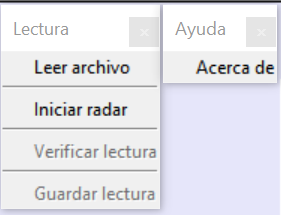
\includegraphics[scale=1.25]{desplegables}
	\caption{Menús desplegables de RadarWave.}
	\label{fig:desplegables}
\end{center}
\end{figure}

Un poco mas abajo llama la atención una barra de herramientas con iconos, esos iconos se corresponden con el menú desplegable de \textit{Lectura}. Cada icono se corresponde con un item del menú.
Los botones de izquierda a derecha se corresponden con las funcionalidades de abrir fichero de lecturas ya generadas, iniciar lectura por radar, clasificar objeto y guardar lectura generada.

La aplicación es capaz de conectar con el radar sin tener que acceder a la configuración de este en ningún momento. Los únicos requisitos son tener conectado el radar a la corriente eléctrica y a la red de internet (mediante \textit{Ethernet} o \textit{Wifi}). La comunicación de la interfaz con el radar se ha generado principalmente con las librerías \textit{Socket} y \textit{Paramiko}.

Dentro del código fuente se han incluido la mayoría de las funciones utilizadas para el tratamiento de las lecturas iniciales de las vistas de los objetos, es decir se realiza una lectura in sito con el radar para extraer los datos del objeto, estos datos se transforman y se tratan con las mismas funciones que fueron encargadas de generar los datos para la creación y entrenamiento del modelo.

El detallado del código de la aplicación se expone dentro del anexo \textit{D - Documentación técnica de programación}.

